\chapter{Permanent pile head rotation}\label{sec_6}


The predicted permanent pile head rotation is shown in Figure ~\ref{perm_rotation}. The permanent pile head rotation represents the plastic part of the pile head response under loading (i.e. the total rotation subtracted by the rotation due to elastic deformation). The permanent pile head rotation for the current pile geometry is less than the allowable limit of 0.300°.

\begin{figure}[!htbp]
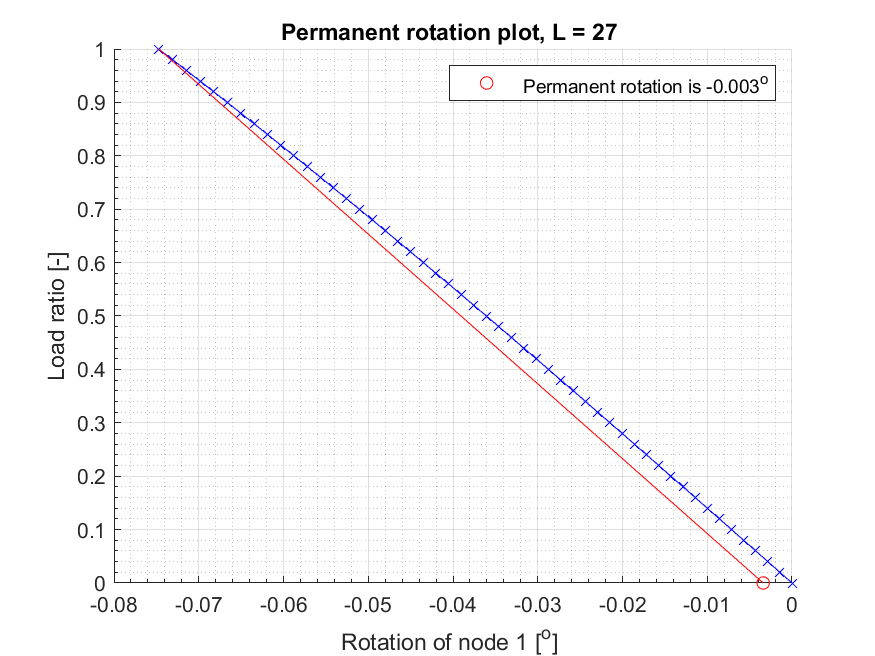
\includegraphics[width=0.9\textwidth]{AppendixGenerationFiles/ProjectLocation/permanent_rot_def.png}
\caption{Permanent pile head rotation for unfactored ULS loading at WTG {\ID_location}. Characteristic soil properties adopted and with the effect of cyclic degradation considered.}
\label{perm_rotation}\end{figure}
